\newpage
\section{Pangénome de séquences}

\subsection{Pangénome basé sur une séquence représentative}

Un pangénome basé sur les séquences correspond à un ensemble de génomes dont l'alignement minimise le nombre de régions homologues tout en rendant compte de toute la diversité. L'objectif derrière ces pangénomes est d'obtenir une séquence pangénomique de référence. De façon contre-intuitive (par rapport à la définition "sans-référence" des pangénomes), pour construire ces pangénomes, on utilise une séquence représentative comme base. Toutes les séquences seront alignées à partir de cette base, et les segments non redondants détectés dans au moins un génome seront intégrés à la référence non redondante (NRR, Non-Redundant Reference en anglais). L'ensemble, séquence représentante et NRRs, forme alors la séquence pangénomique de référence.

\subsubsection{Méthode de construction}

Pour construire ces pangénomes, il faut d'abord identifier une séquence représentative. Les autres séquences, en général des séquences non assemblées (lectures ou \textit{reads} en anglais), sont alignées contre la représentante et les séquences non alignables sont considérées comme des NRRs potentiels. Les NRRs de taille inférieure à 500 pb sont exclues, ainsi que celles dont la similarité avec la représentante est supérieure à un seuil (90 \% en général). Les NRRs restantes sont comparées à des bases de données pour retirer tous les contaminants potentiels. De ce schéma général, on peut identifier 4 méthodes différentes pour l'identification des NRRs potentiels :
\begin{itemize}
    \item \textbf{Assemblage de type métagénomique} : les lectures non alignées sur la référence sont regroupées et assemblées \textit{de novo}. Les contigs obtenus sont ajoutés à la séquence représentante. Cette méthode est efficace même avec une faible couverture des lectures.
    \item \textbf{Assemblage itératif} : Dans un premier temps, les lectures non alignées du premier échantillon sont assemblées et ajoutées au génome de référence. Ce génome mis à jour sert ensuite de base pour l’assemblage des échantillons suivants. Ce processus est répété pour tous les échantillons.
\end{itemize}
\newpage
\begin{itemize}
    \item \textbf{Assemblage indépendant des \textit{reads} non alignés} : Toutes les lectures non alignées sont séparées par échantillon\footnote{Ensemble de lectures obtenues simultanément} et assemblées \textit{de novo} indépendamment. Les contigs obtenus sont regroupés selon leur similarité. Dans chaque groupe, un contig référent est identifié et est intégré à la séquence référente. Cette méthode nécessite une couverture d’au moins 10×, pour obtenir des contigs de taille suffisante.
    \item \textbf{Assemblage génomique indépendant} : chaque échantillon est assemblé indépendamment, et les contigs obtenus sont alignés à la référence. Les contigs non alignés sont regroupés par similarité et un contig référent est ajouté à la séquence référente.
\end{itemize}

Le choix de la méthode dépend du type et de la quantité des données disponibles. Avec une faible couverture (<10×) et un grand nombre d’échantillons, l’approche métagénomique est recommandée, bien qu’elle puisse produire des contigs chimériques. Avec une couverture plus élevée (>10×), l’assemblage indépendant ou l’approche itérative sont préférables. Cette dernière est plus lente, mais facilite l’ajout de nouveaux échantillons. Enfin, si plusieurs assemblages de haute qualité existent déjà, l’assemblage génomique indépendant est la meilleure option. Ces méthodes peuvent être combinées pour optimiser l’utilisation des données disponibles.
 
\subsubsection{Domaines d'application des pangénomes basés sur une séquence représentative}

Ces pangénomes sont particulièrement utiles lorsque les données de départ sont des \textit{lectures}. En utilisant ces modèles, il est possible de revenir à une séquence linéaire qui peut être utilisée dans les outils classiques de génomique. De plus, il peut également être utilisé comme étape préliminaire à la construction d'autres types de pangénomes, en réduisant rapidement la redondance dans un sous-ensemble proche de génomes. 

L'outil NGSPanPipe \cite{kulsum_ngspanpipe_2018} est un pipeline intégré conçu pour l'identification du pangénome à partir de lectures courtes (short reads) issues du séquençage de nouvelle génération (NGS). Contrairement à d'autres méthodes nécessitant des prétraitements des lectures, NGSPanPipe permet une analyse directe des reads bruts pour identifier le pangénome. Il ne génère pas de séquence pangénomique linéaire, mais il permet de reconstruire des contigs à partir des lectures en utilisant un génome de référence. Les contigs obtenus à partir des lectures alignées, permettent de calculer la couverture du génome par rapport au pangénome. Les lectures non alignées sont comparées à des bases de données de \textit{reads} pour identifier de nouveaux \textit{reads}, puis ils sont assemblés en contigs. L'ensemble des contigs (de lectures alignées et non alignées) sont annotés et utilisés pour construire une matrice binaire représentant la présence ou l'absence des gènes dans la séquence de référence.

\subsection{Pangénome graphe}

Les graphes de séquences sont un modèle de pangénome permettant de visualiser la diversité génomique, qu’elle soit basée sur une séquence de référence ou non. Dans tous les cas, des segments de séquences vont constituer les n\oe uds du pangénome et les arêtes seront étiquetées par des informations permettant de retrouver le lien entre les segments (comme l'organisation dans les génomes). Ce modèle pangénomique a l'intérêt de représenter toute la diversité, codant et non codant. 

\subsubsection{Méthodes et outils de construction}

\paragraph{Graphe de variant prédéterminé}

La première méthode de construction des graphes de pangénome se base sur l'utilisation d'une séquence référente et d'un fichier contenant les variations connues dans les autres séquences par rapport à cette référence. Cette méthode a l'intérêt de demander peu de ressources, car les variations sont prédéterminées et données en entrée. Toutefois, pour obtenir un graphe fiable et précis, un génome complet de bonne qualité est requis.

L'outil VG (\textit{Variation Graph toolkit}) \cite{garrison_variation_2018}, contient un ensemble d'outils permettant de générer un graphe de variants. À partir de ce graphe, qui peut être assimilé à un graphe de pangénome, il est possible de détecter les variants structuraux (SVs) et les SNPs rapidement. Le graphe est indexé, rendant les recherches et l'alignement plus efficaces, notamment dans l'alignement de lectures ou dans la recherche de variants génétiques (\textit{variant calling}). L'outil a d'abord été développé pour la génomique humaine, mais il est tout à fait possible de l'utiliser avec des génomes procaryotes.

L'outil Minigraph \cite{li_design_2020}, lui aussi développé pour le variant calling sur le génome humain, propose une méthode demandant moins de ressources que VG. Le graphe est plus léger, sans annotation, permettant de construire des graphes de pangénome de grande taille, en utilisant peu de mémoire de calcul et de stockage. Minigraph permet de capturer les grandes variations génomiques, mais est moins performant sur la détection des SNPs par rapport à VG.

\paragraph{Graphe d'alignement multiple}

Une méthode, proche de la précédente, est celle basée sur l'alignement multiple des séquences (MSA\footnote{cf. \autoref{paragraph:MSA}}) entre elles. Cette méthode n'est pas dépendante d'une séquence référente. Le MSA permet de déterminer les variations entre les séquences, ce qui augmente le coût en ressources par rapport au graphe de variants prédéterminé. Toutefois, cette méthode est plus adaptée dans le cas où plusieurs séquences de bonne qualité sont disponibles pour construire le pangénome. En effet, le MSA permet de se passer du biais de la séquence référente dans la construction du graphe et d'ainsi mieux représenter la diversité génomique.

L'outil Harvest \cite{treangen_harvest_2014}, permet de comparer des génomes étroitement apparentés. Pour optimiser l'étape d'alignement, il utilise l'outil progressiveMauve \cite{darling_progressivemauve_2010}, qui fait un alignement progressif des séquences. Après l'alignement, il identifie le \textit{core genome} dans le pangénome et génère une phylogénie basée sur une matrice des SNPs. Bien qu'étant rapide et efficace, il n'est pas adapté aux génomes très divergents et il ne permet pas d'analyser les éléments mobiles (MGE).

PGGB \cite{garrison_building_2024}, utilise des algorithmes de graphes de préfixes minimaux (MPHF\footnote{Minimal Perfect Hash Function (MPHF) est une fonction qui associe de manière unique chaque élément d’un ensemble sans collisions et avec un espace mémoire minimal}), pour compresser le graphe et optimiser l'alignement. Il est capable d'identifier et de représenter les SNPs, SV, et les MGEs de manière efficace. PGGB est conçu pour mener des études pangénomiques à grande échelle, prenant en compte de grandes quantités de séquences, ce qui demande des ressources disponibles importantes. De plus, c'est un outil assez complet pour les analyses, ce qui peut le rendre difficile d'accès.

\paragraph{Graphe de De Bruijn}

Les graphes de De Bruijn (De Bruijn Graph : DBG) sont des graphes orientés dont les n\oe uds représentent des k-mers et les arêtes le chevauchement entre le suffixe et le préfixe (de taille k-1) des k-mers (\autoref{fig:deBruijn}). Ainsi, en suivant un chemin, il est possible de reconstituer une séquence. C'est pourquoi les DBG sont utilisés dans de nombreuses applications en bioinformatique (assemblage, correction des erreurs de séquençage, métagénomique\dots) et notamment en pangénomique.

\begin{figure}[htbp]
    \centering
    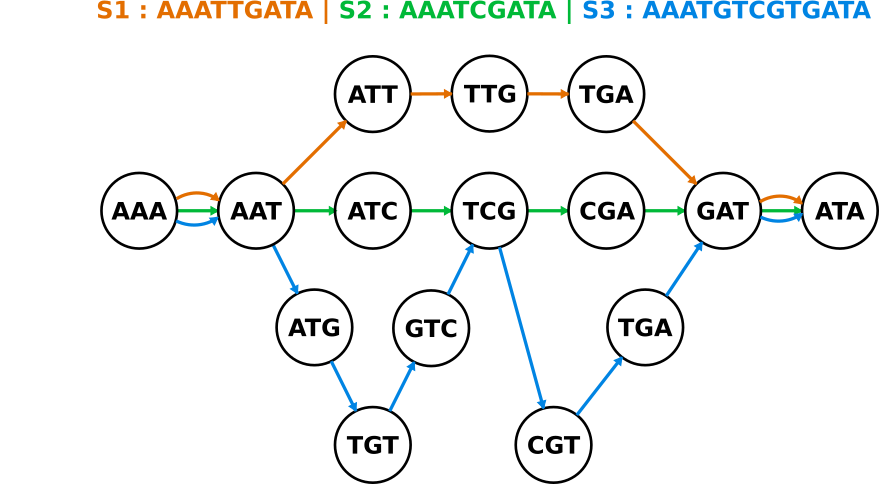
\includegraphics[width=.9\linewidth]{images/DBG.png}
    \caption[Exemple d'un graphe de De Bruijn]{\textbf{Exemple d'un graphe de De Bruijn.} Ici $k=3$, ce graphe permet de représenter et de reconstruire 3 séquences.}
    \label{fig:deBruijn}
\end{figure}

Les DBG, permettent d'avoir une structure compacte des séquences du pangénome. Les n\oe uds et les arêtes sont colorées en fonction des génomes dans lesquels ils sont retrouvés. Les DBG peuvent être compactés en cDBG, en fusionnant chaque région \textit{core}, \textit{i.e.} chaque suite de n\oe uds avec une seule arête entre chaque n\oe ud. Ces nouveaux n\oe uds fusionnés sont appelés "\textit{unitig"} et seront étiquetés avec la séquence combinée des k-mers.

L'une des premières méthodes développées utilisant des DBG, est la méthode Cortex \cite{iqbal_novo_2012}, qui construit un DBG "coloré" (les arêtes et les n\oe uds sont étiquetés par les échantillons dans lesquels ils sont trouvés). À partir de ce DBG coloré, il est possible d'identifier les variants et de les associer à un génotype. Des outils plus récents, comme Bifrost \cite{holley_bifrost_2020}, améliorent les méthodes de coloration de DBG, permettant d'augmenter le volume de données pris en compte et supportant la mise à jour du graphe. Les auteurs de Bifrost ont notamment appliqué leur méthode sur une collection de plus de 100 000 génomes de \textit{Salmonella} \cite{luhmann_blastfrost_2021}, leur permettant d'identifier des gènes reliés à des îlots de pathogénicité et à une résistance aux fluoroquinolones\footnote{Classe d'antibiotique utilisée pour traiter les infections bactériennes graves.}.

\newpage
SplitMEM \cite{marcus_splitmem_2014}, permet de construire rapidement et efficacement des cDBG en intégrant une méthode appelée "saut de suffixe"\footnote{Le cDBG est relié à des arbres de suffixes, un saut de suffixe permet depuis un suffixe à l'extrémité d'une branche de l'arbre de sauté vers un même suffixe plus proche de la racine. Les sauts se poursuivent jusqu'à atteindre le suffixe le plus proche de la racine. Le chemin restant correspond au chemin le plus court sans ramification, entre la racine et le suffixe.}, qui permet de construire le cDBG sans passer par un DBG. L'outil permet ensuite de détecter dans l'ensemble des génomes ou dans un sous-ensemble de génomes les régions compressées (appelées \textit{Maximum Exact Matches} : MEMs), correspondant au \textit{core genome}. Cet outil est linéaire en temps et en espace pour identifier le \textit{core genome}, mais ne permet pas de mener d'autres analyses. De plus, la méthode a été testée sur un jeu de 62 génomes de \textit{E. coli}, le caractère linéaire est donc à vérifier sur de plus grands jeux de données.

PanTools \cite{sheikhizadeh_pantools_2016}, est un outil complet qui a largement évolué depuis sa publication. Il permet la construction de pangenomes basés sur des cDBG généralisés. PanTools est robuste à l'utilisation de grands volumes de données, que ce soit en temps, en mémoire ou en stockage. Il intègre également des méthodes d'annotation structurale et fonctionnelle, de partitionnement, d'alignement, de phylogénie, d'identification du \textit{core genome} et de visualisation. 

DBGWAS \cite{jaillard_fast_2018}, construit également les pangénomes avec des cDBG. Son originalité réside dans l'association de phénotypes (\textit{Genome Wild Association Study} : GWAS). L'intérêt d'utiliser le graphe de pangénome est qu'il n'est pas nécessaire d'utiliser une séquence de référence, contrairement aux approches classiques de GWAS. De plus, les phénotypes ne sont pas associés à des SNPs mais à des sous-graphes, permettant d'extraire des variants plus longs ou plus complexes. DBGWAS intègre une partie visualisation, permettant d'explorer les variants associés au phénotype dans leur contexte génomique pour identifier des régions variables plus larges comme les îlots génomiques. 

Le DBG (et ses dérivés) est une structure de données puissante, permettant de calculer, analyser et stocker, rapidement et efficacement, de grandes quantités de données. Néanmoins, ce qui fait la force de cette approche (l'utilisation de k-mer) est aussi sa faiblesse. Le choix de la taille du k-mer va influencer le graphe et donc la découverte des variations. De plus, cette structure est limitée dans l'identification et l'étude des régions répétées. C'est pourquoi des auteurs proposent des méthodes pour lier des informations au DBG \cite{turner_integrating_2018}.

\subsubsection{Application des graphes de pangénome.}

L'utilisation de pangénomes de séquence est très utile à partir de lectures courtes pour améliorer le génotypage. En utilisant le pangénome, contenant des variants connus, on améliore la couverture des lectures et donc on améliore le génotypage de ces lectures. Par rapport aux méthodes utilisant un génome de référence, le pangénome réduit le biais en faveur de la séquence de référence, particulièrement pour les grandes insertions/délétions et les SV. Le pangénome améliore aussi le \textit{variant calling} (VC) en augmentant sa précision, et à partir des DBG de faire du VC sans référence.

Les graphes de séquences sont également utilisés en métagénomique. L'outil MetaKallisto \cite{schaeffer_pseudoalignment_2017} utilise notamment une base de données de séquences représentantes qu'il représente sous forme de DBG coloré afin de faire de l'assignation taxonomique et de la quantification de séquences métagénomiques.

L'utilisation des graphes de séquences pour les GWAS permet de détecter finement des variations dans les populations associées à un phénotype. Chaguza \textit{et al.} \cite{chaguza_bacterial_2020} ont mené une étude sur 909 échantillons de souche hyper virulente de \textit{Streptococcus pneumoniae} (serotype 1). Ils ont pu identifier, grâce à l'outil DBGWAS, des mutations de certaines protéines associées à des phénotypes spécifiques (âge de l'hôte, géographie, structure des populations\dots). L'utilisation de graphes de pangénome a permis de mener une étude à large échelle, tout en prenant en compte toute la diversité sans nécessiter de référence.

\begin{table}[htbp]
    \centering
    \begin{tabular}{|p{.25\textwidth}|p{.3\textwidth}|p{.35\textwidth}|}
        \hline
        Nom & Méthode & Référence \\
        \hline
        NGSPanPipe & Séquence représentative & \cite{kulsum_ngspanpipe_2018} \\
        \hline
        Spine & Séquence représentative & \cite{ozer_characterization_2014}\\
        \hline
        VG toolkit & Variant prédéterminé & \cite{garrison_variation_2018} \\
        \hline
        Minigraph & Variant prédéterminé & \cite{li_design_2020} \\
        \hline
        PanVC & Variant prédéterminé & \cite{norri_founder_2021} \\
        \hline
        Minigraph-Cactus & MSA & \cite{hickey_pangenome_2024}\\
        \hline
        Harvest & MSA & \cite{treangen_harvest_2014} \\
        \hline
        PGGB & MSA & \cite{garrison_building_2024}\\
        \hline
        Cortex & graphe de De Bruijn & \cite{iqbal_novo_2012} \\
        \hline
        Bifrost & graphe de De Bruijn & \cite{holley_bifrost_2020} \\
        \hline
        SplitMEM & graphe de De Bruijn & \cite{marcus_splitmem_2014} \\
        \hline
        PanTools & graphe de De Bruijn & \cite{sheikhizadeh_pantools_2016} \\
        \hline
        twoPaCo & graphe de De Bruijn & \cite{minkin_twopaco_2017}\\
        \hline
        DBGWas & graphe de De Bruijn & \cite{jaillard_fast_2018}\\
        \hline
        PanVA & Visualisation & \cite{van_den_brandt_panva_2024} \\
        \hline
        
    \end{tabular}
    \caption[Outils de pangénomique basés sur les séquences]{\textbf{Liste non exhaustive d'outils de pangénomique basés sur les séquences.}}
    \label{tab:pangenomicToolsSeq}
\end{table}